\documentclass{article}
\usepackage{ctex}
\usepackage[a4paper]{geometry}
\usepackage{amsthm,amsmath,amssymb}
\usepackage{ulem}
\usepackage{graphicx}
\usepackage{gensymb}
\usepackage{url}
\usepackage{hyperref}
\usepackage{enumitem}
\usepackage{color}

\begin{document}
\normalem
\section{层次数据可视化}
数据可视化中的很多数据都是具有层次结构的,比如说电脑中的文件、公司组织机构等等。一些多维数据尽管没有层次信息,
有时候还是需要通过按照不同的维度分组来分析不同维度的属性上的关系,不同的分组方法就会产生不同的层次结构。
现有的数据可视化方法大体上可以分为两类:基于Node-Link的方法和基于Space-Filling的方法。
\subsection{方法角度}
基于Node-Link的方法有:
\begin{itemize}
	\item Node-Link Tree:Tree是图的一种特例,是描述层次结构最常用也最直观的方式,但是在描述层次结构的数据时候,随着层数的增加,
		节点数目(大多数情况下)呈指数增长,所以如果采用top-down的布局,接近root的地方节点稀疏,越向下节点越密集,这使得空间利用率不高。
		当在每个节点上附加一个说明性的label时,很容易出现重叠,尤其是在低层元素较多时候更加明显。

	\item Hyperbolic Tree(图\ref{fig:hyperbolic_tree}): 将子节点空间限制在父节点所在位置所形成的双曲线空间内。

	\item Radial-Tree(图\ref{fig:radial_tree}):
		Radial-tree,放射形的元素排列,所有叶子节点被放置在一个同心圆上,相比node-link diagram的空间利用率高,但是由于元素不在一个平面上,
		很难区分一组元素是不是在同一个层次上,所以进行同一层次元素属性比较的时候不是很直观。cone tree将radial-node-link扩展到三维空间。
		TimeRadarTrees\cite{Burch2011TimeRadar}是Radial layout的一个应用。

	\item Layered Icicle Plot:
		需要较大的图片空间,父亲元素所需要的空间约等于子元素空间的总和,但好处就是展示的结构比较清晰,很容易向某一放下扩展。

	\item Sunburst布局,使用了和Treemap相似的方法,不同的是Treemap是基于矩形的布局,Sunburst一个环形(放射形)的布局方式。
		Sunburst图可以看作是径向的icicle plot。Sunbirst图在层次较深将诶点较多的时候会有thin-slice的问题,外层的元素成为窄条形不易辨认,
		文章中提出了用一种fisheye distortion的交互方式来解决thin-slice问题。

	\item H-Tree(图\ref{fig:h-tree})是一种分形的树可视化,节点具有自相似的特性,适用于二叉树的可视化,广泛应用在VLSI设计中\cite{browning1980tree}。

	\item \cite{munzner2003treejuxtaposer}addresses the problem of comparing
		trees with more than a hundred thousand nodes, a range that is typical for phylogenetic trees,
		which are explored in the field of biology or bioinformatics.
		The researchers introduce the concept of guaranteed visibility--highlighted elements have
		to be trackable all the time during the exploration process

\end{itemize}


\begin{figure}[h]
	\centering
	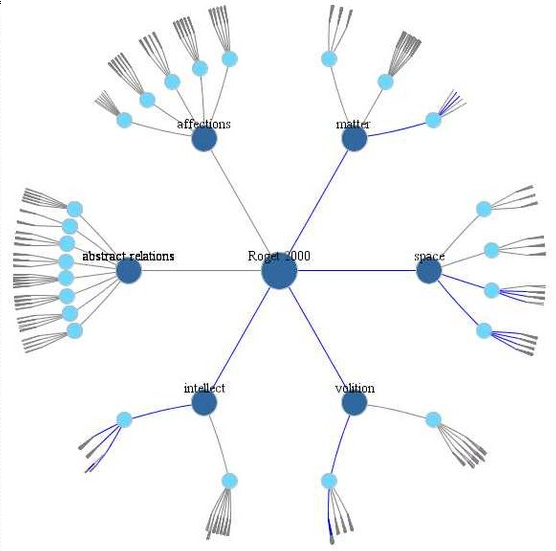
\includegraphics[width=0.5\textwidth]{_img/hyperbolic_tree.png}
	\caption{Hyperbolic Tree}
	\label{fig:hyperbolic_tree}
\end{figure}

\begin{figure}[h]
	\centering
	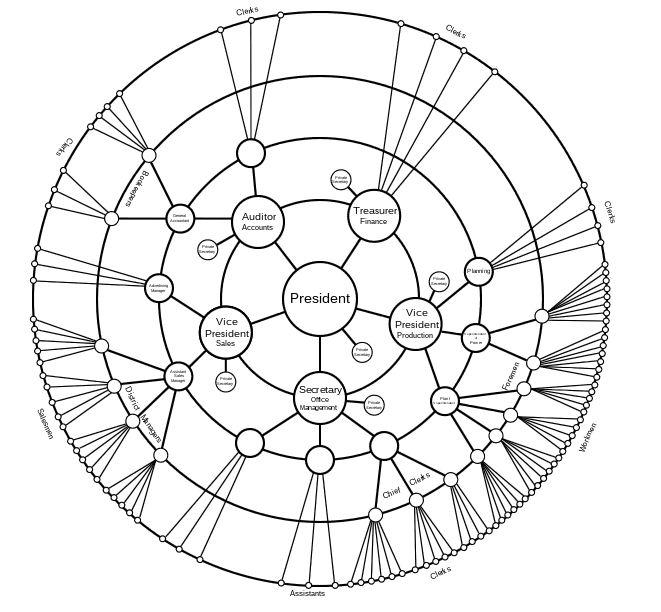
\includegraphics[width=0.5\textwidth]{_img/Radial_Tree.png}
	\caption{Radial Tree}
	\label{fig:radial_tree}
\end{figure}

\begin{figure}[h]
	\centering
	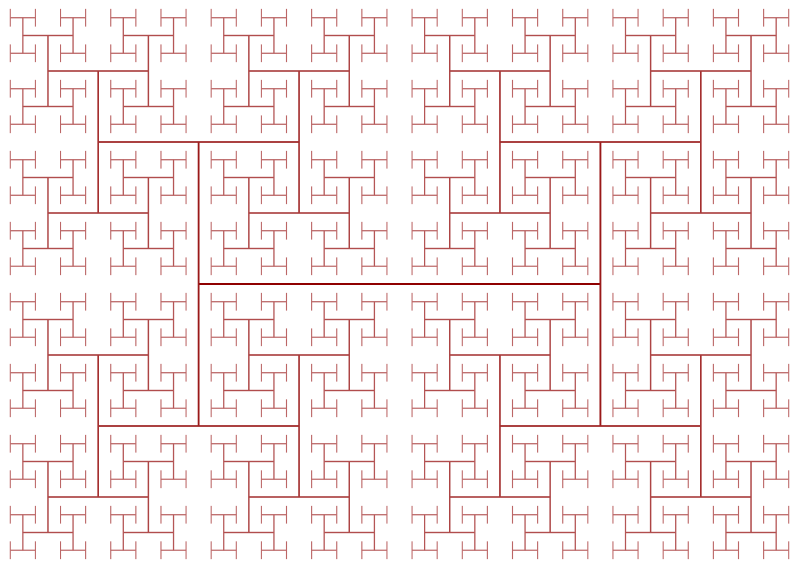
\includegraphics[width=0.5\textwidth]{_img/H-Tree.png}
	\caption{H-Tree}
	\label{fig:h-tree}
\end{figure}


基于Space-Filling的方法有:
\begin{itemize}
	\item Treemap:
		Treemap是在1991年由Bran Johnson和Ben Shneiderman在文章中提出的。Treemap能够最大限度的利用空间资源,但是对层次信息的展示不是很明显。
		在可视化层次结构的数据时,treemap是个很好的选择,缺点在于整个数据的层次结构不会太清晰,这个问题虽然可以通过矩形边框特殊化的方式解决,
		但是会浪费一定的空间,而且当层次结构复杂的时候效果也不会很好。如果数据层次较深且数据较多,低层的元素可能会退化成接近像素点矩形,不容易辨认。
		常用的解决方法是通过将低层次的元素聚合到高层次的的元素,同时提供显示聚合元素信息的交互手段。

	\item Cushion Treemap(图\ref{fig:cushion_treemap}):
		Cushion Treemap最早在文章\cite{Wijk1999}中提出,目的是为了弥补treemap对层次信息显示不好的缺点。
		cushion treemap加入了阴影效果来增强层次结构信息,同时每个矩形通过脊状线(ridges)来增强层次感。

	\item Squarified Treemap(图\ref{fig:squarified_treemap}):
		文章\cite{Bruls99squarifiedtreemaps}中提出的算法用于解决原始的treemap算法:slide-and-dice算法,会产生细长的矩形无法识别的问题。
		这个算法生成的treemap具有良好的横纵比(aspect ratio),所有矩形接近方形便于识别。

	\item Voronoi Treemap(图\ref{fig:voronoi_treemap}):
		Voronoi Treemap\cite{Balzer_voronoitreemaps}将treemap扩展,内部分割和外部区域可以使用任意多边形而不局限于使用矩形。

	\item Balloon\cite{boardman2000bubble} or Bubble diagram:深层节点所占的空间会比较小,
		不适合用在大量数据或层次较多的数据上,而且不方便比较不属于同一分支的数据元素。

	\item 其他:
		\begin{itemize}
			\item Bubblemaps and Quantum Treemap
			\item Ordered Treemap
			\item Clustered Treemap
			\item Cascaded Treemap
			\item Modifierable Treemap
			\item Circular Treemap
		\end{itemize}
		Treemap 历史\cite{treemaphistory}
	\item Variable Zoom\cite{schaffer1996navigating}通过cluster将部分节点聚合到高层节点上,从而减少了可视节点的数量避免信息重叠,
		应用focus+contex的技术来查看高层聚合节点。

	\item ArcTrees(图\ref{fig:arctrees}):
		\cite{neumann2005arctrees}中提出的arctree方法可以用户可视化层次结构信息也可以用来显示非层次结构信息。
		一般来说在一个可视化中同时显示层次信息和关系信息是比较难的,因为这样很容易让用户产生误解。
		论文提出的方法从传统的treemap派生而来,通过在treemap上增加弧线来表示关系。
		用户可以通过一些交互来探索数据特征,通过focus+context技术浏览整个视图。
		最初的想法是用来可视化文档结构关系,但是也可以用作工程管理和日历中。

	\item \cite{andrews1998information}被看作是Sunburst的先驱,\cite{stasko2000focus}提出Sunburst

\end{itemize}

\begin{figure}[h]
	\centering
	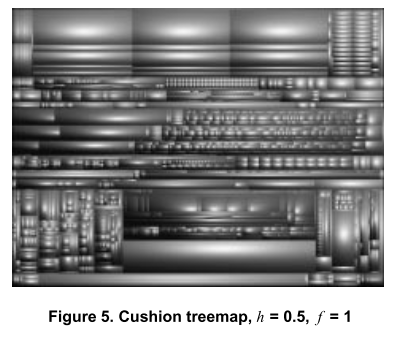
\includegraphics[width=0.5\textwidth]{_img/Cushion_Treemap_.png}
	\caption{Cushion Treemap\cite{Wijk1999}}
	\label{fig:cushion_treemap}
\end{figure}

\begin{figure}[h]
	\centering
	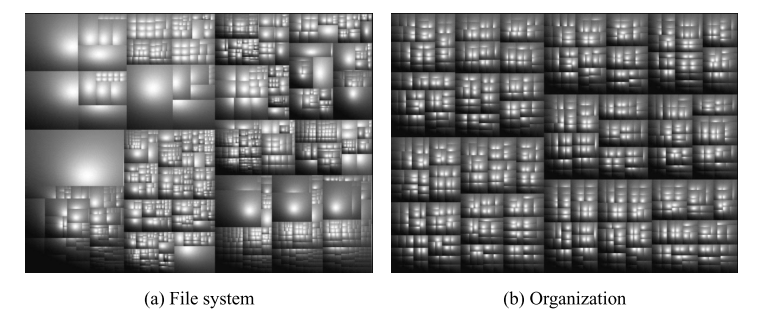
\includegraphics[width=0.5\textwidth]{_img/Squarified_Treemap_.png}
	\caption{Squarified Cushion Treemap\cite{Bruls99squarifiedtreemaps}}
	\label{fig:squarified_treemap}
\end{figure}

\begin{figure}[h]
	\centering
	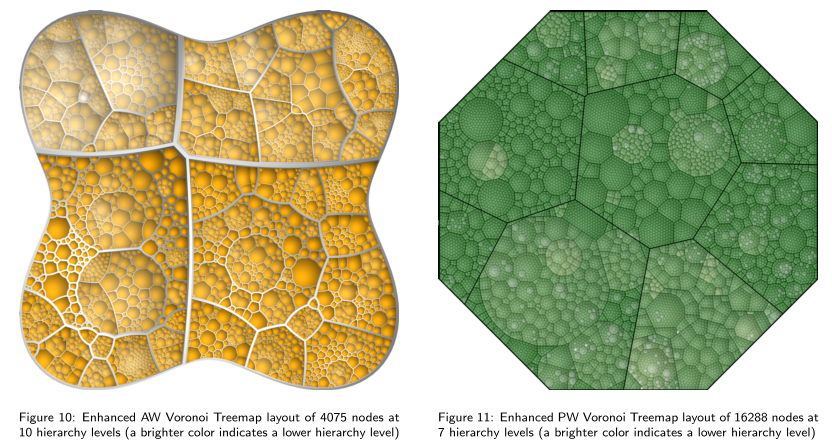
\includegraphics[width=0.5\textwidth]{_img/Voronoi_Treemap_.png}
	\caption{Voronoi Treemap\cite{Balzer_voronoitreemaps}}
	\label{fig:voronoi_treemap}
\end{figure}

\begin{figure}[h]
	\centering
	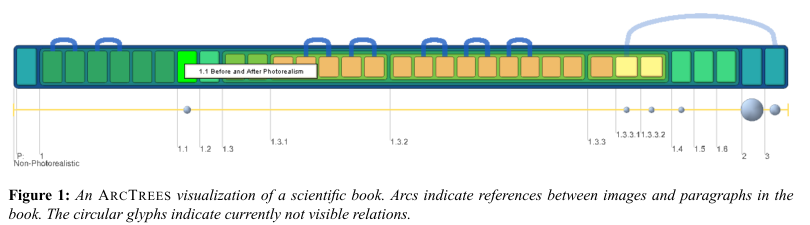
\includegraphics[width=\textwidth]{_img/ArcTrees_.png}
	\caption{ArcTrees\cite{neumann2005arctrees}}
	\label{fig:arctrees}
\end{figure}

混合方法:

\subsection{分析角度}
根据不同的数据,用户所关注的点可能不同,可能关注数据的\emph{Structure/Attributes}
也有可能是\emph{宏观特点/微观特点},还有可能是\emph{静态特性/动态特性}。

\subsection{动态层次数据}
在动态时序数据可视化方法中,最自然的方法应该是把数据按照时间顺序映射到一系列图上,用动画的方式展现。这种方式依赖于用户能够记住多少图中元素的变化,
所以需要不断的重复播放直到用户能够发现元素变化的特点。所以用动画的方式会极大的增加用户的认知负担,需要寻求时序数据的静态表示方法,
同时充分利用交互的手段作为辅助。

Treemap用在动态层次数据可视化上一般是通过将treemap的显示属性和数据的属性相关联的方式实现的,
比如矩形的大小(所占比例)或颜色,底纹等等都可以用来作为数据属性的隐喻。用treemap可视化层次数据可以很好的展示最低一层数据的属性块,
当treemap用于静态的层次结构数据分析来发现数据属性之间的关联时,用来进行分组的属性的顺序会比较重要,不合理的分组顺序会产生毫无意义的结果,
,所以要根据数据的特点进行合理的分组。

\subsection{动态层次数据可视化的论文}
\begin{itemize}
	\item \cite{burch2011} 
		用正交的直线连接父子节点,在直线上叠加信息展示时序数据,一般通过颜色和厚度编码信息。
		(We exploit the straight links of orthogonal tree diagrams as a
		timeline on which we visually encode dynamic quantitative
		information.  We use color coding and varying thicknesses to
		represent the time-varying data.)
	\item \cite{sirin2002} {\sout{在Treemap3中显示非层次信息,允许用户自定义数据的层次结构,通过不同的组合帮助用户发现数据中的隐藏信息。}}

	\item \cite{theron2006hierarchical}用类似于年轮的布局方式展示时序层次数据,用到了focus+contex的交互方式。(图\ref{fig:tree_ring})

	\item \cite{wilson1999dynamic}在把非层次数据层次化的时候,分组的顺序很重要,论文提出的方法允许用户定义数据的层次,
		提供multi-hierarchical layout、layout blending、dynamic partition adjustment等技术帮助用户选择合理的层次化顺序从而发现数据中的信息。
		同论文\cite{sirin2002}有点类似。

	\item \cite{stasko2000focus}放射状sapce-filling可视化方法在层次增多时许多数据条目会变得非常小,
		这篇论文提出了三种可视/交互方法帮助用户在保持一个层次的全局图的情况下辨别这些信息。
		\begin{enumerate}
			\item Angular Detail Method:将需要显示的部分放大,全局图缩小。
			\item Detail Outside Method:全局图缩小到中间,要放大显示的部分扩大成圆环包裹全局图。
			\item Detail Inside Method:显示部分放中间
		\end{enumerate}
		并分析了三种方法的优缺点。
	\item \cite{TVCG2322594}2014发表在TVCG上的文章,引入邻接链表(邻接矩阵)的概念来可视化动态图。用颜色和label区分节点,大小表示权重。
		在边上采用了非对称的映射方式。
\end{itemize}
\begin{figure}[h]
	\centering
	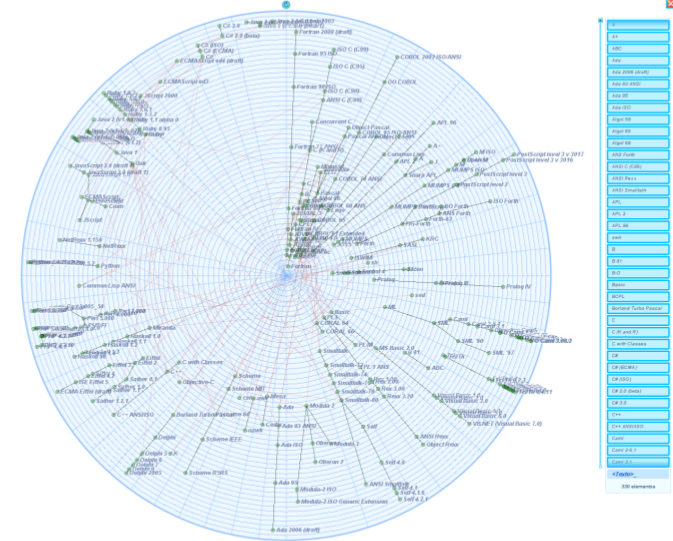
\includegraphics[width=0.5\textwidth]{_img/tree_ring.png}
	\caption{用tree ring可视化计算机语言的发展演变}
	\label{fig:tree_ring}
\end{figure}
\section{论文}

\cite{burch2011}基于node-link的tree,parent-child关系用连接两个node的正交直角线表示,连线同时当作时间线,
在时间线上附加具有颜色和厚度的矩形来表示节点的属性随时间的变化信息。可以用来展示数据的五种不同行为:
trends, contertrends, periodicity, temporal shifts, anomaly,(图\ref{fig:burch2011.png})
\begin{figure}[h]
	\centering
	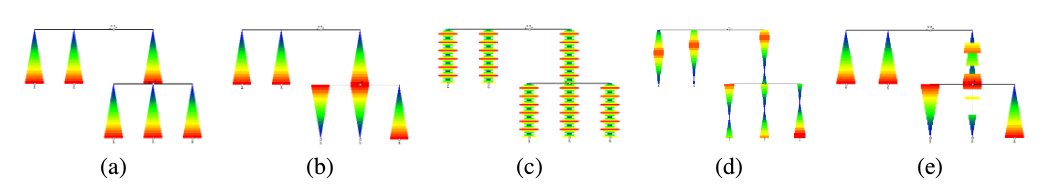
\includegraphics[width=\textwidth]{_img/burch2011_.png}
	% \caption{Burch2011}
	\label{fig:burch2011.png}
\end{figure}

文章\cite{JHS2011}提出了层次数据可视化的design space,包括四个方面:
\begin{enumerate}
	\item 维度:2D or 3D
	\item 点的表示:用什么图像元素
	\item 边的表示:用包含、重叠还是邻接的方式表示parent-child关系
	\item Layout方法:是用细分(subdivision)还是包装(packing)的方式构建layout
\end{enumerate}
,说明了现有的大多数层次数据可视化方法都可以基于treemap和icicle plot从以上四个方面通过不同的组合得到。

\begin{itemize}
	\item 文章\cite{frank1998different}对时序数据可视化中不同的时间轴表示进行了分类:
		\begin{itemize}
			\item 周期时序 vs. 线性时序(cyclic vs. linear time)
			\item 离散时间 vs. 时间区间(discrete time point vs. interval)
			\item 序数时间 vs. 连续时间(ordinal vs. continuous time)
			\item 有序时间 vs. 时间分支 vs. 时间多视角(ordered vs. branching time vs. time with multiple perspective)
		\end{itemize}
	\item \cite{muller2003visualization}是一个基于时间的可视化技术的综述。
		作者将基于时间的可视表现划分为静态的、动态的以及基于事件的。动画效果的展示容易让用户产生对数据的误解。
		有两个可选的静态趋势可视化,
		\begin{itemize}
			\item multaneously overlaid trends in one single display
			\item a small multiples display that shows trends side-by-side
		\end{itemize}
\end{itemize}

\section{层次数据可视化的例子}
\begin{itemize}
	\item \cite{balzer2005voronoi}用Voronoi Treemap\cite{Balzer_voronoitreemaps}分析软件。
	\item \cite{vliegen2006visualizing}用通用(generalized)的treemap来分析商业数据。
	\item \cite{jin1997tennisviewer}用来分析网球比赛
	\item \cite{jungmeister1992adapting}把treemap用在股片市场portfolios来帮助进行商业决策。
	\item \cite{wattenberg1999visualizing}把treemap应用在公开的商业公司数据上,见网站
		\emph{SmartMoney Map of the Market}
\end{itemize}

\section{TODO}
\begin{itemize}
	\item 看论文总结:
		\begin{itemize}
			\item 层次数据可视化的例子(系统)
			\item 根据不同的数据特点,分析其所用的可视化基本方法以及技巧
			\item 文章是如何组织的
		\end{itemize}
	\item 详细分析信号树数据,
		\begin{itemize}
			\item 把radial tree做成可展开折叠的
			\item 旁边加一个显示节点流量的视图,在选中节点时显示相应的信息 
		\end{itemize}
\end{itemize}
\bibliographystyle{plain}
\bibliography{ref_summary}
\end{document}
